\chapter{Supernova Remnants: Theory and  Observation}
\label{chap:Rems}

\section{Introduction}\label{Rems:intro}
When a massive star at the end stage of its evolution explodes as a supernova, it nearly instantaneously injects a massive amount of kinetic energy into the surrounding medium ($\sim 10^{51}$ erg). The supersonically expanding blast-wave, ejected stellar mass, and possible compact stellar remnant comprise an \snr{}. The first two identified \snrs{} (the Crab and Kepler's \snr{}) were initially observed as optical nebulosities found to be associated with historical supernovae. It was not until the advent of the radio interferometer that a number of these nebulae were discovered and could thus be studied as a population.  In fact, one of the first discrete radio objects to be detected was a remnant in the Cassiopeia constellation now known as Cassiopeia A \citep{Ryle48}. \jamie{find some kewl SNR pics, (maybe the first crab one?) if I have time }

One of the primary distinguishing features of the radio emission from \snrs{} was their distinctly non-thermal spectra (a \pl{} with flux ${\rm S \propto \nu^\alpha}$). The clearly non-thermal emission was first proposed to arise from \sync{} radiation (and hence emitted by a population of relativistic electrons) by \cite{Kiepenheuer50} and \cite{Alfven50}, and then by \cite{Shklovskii53} who correctly associated the remnants with supernovae in the Galaxy. To this day, \snrs{} are still primarily identified through radio observations (although a number have been first detected in X-ray as well). A catalog of 294 radio-identified Galactic \snrs{} is maintained at \url{http://www.mrao.cam.ac.uk/surveys/snrs/} by \cite{Green14} (referred to as Green's catalog) and a complementary high-energy catalog, summarizing \snr{}  X-ray to \gam{} properties, is upkept by \cite{Ferrand12} at \url{http://www.physics.umanitoba.ca/snr/SNRcat}


\section{\label{Rems:evo}Formation and Evolution}

-Stars die and explode, that energy is very quickly put into the surroundings
    
-snowplough, ST, radiative,
    
- what else?

How we detect gamma-rays from SNRs/PWNe in the Galaxy leads to and analysis section maybe?
\section{\label{Rems:obs}Morphology and Classification}

SNRs characterized by morphology and evolution properties

shell type, mixed morphology, filled center  composite )

Since I eventually do these all plane surveys, what does the spatial  distribution of them at radio look like?

Not sure how much to say about radio observations, x-ray, TeV

\section{\label{Rems:CR}Cosmic Ray SNR connection}

Give the whole, if 10\% of energy of SN explosion goes into particle acceleration, we can explain cosmic rays

Particle acceleration and DSA

This leads to gamma-ray section

zwicky bade, 

\section{\label{Rems:latGam}Supernova Remnants at \gam~Energies}

By the end of the its science run, \egret{} had detected 271 sources above 100\mev{}, within a minimum detection significance of 4$\sigma$, 170 of which had no clear multiwavelength counterpart, with 81 of those unidentified lying within \blat of the Galactic plane \citep{Hartman99}. The main hindrances to source identification were the numerous potential source counterparts (the \egret{} \psf{} was energy dependent, with a 68\% containment radius of ${\rm \sim 6 ^\circ}$ at 100\mev{} and smaller for higher energies) and the large \egret{} error boxes. In addition to this, the primary method for identifying a \gam{} source as an \snr{} is through a compatible angular extent with  observations at some other wavelength, thus the ability to resolve emission from an \snr{} is vital to understanding the mechanisms therein giving rise to \gam{}s. Figure \ref{fig:3EGSky} shows an \egret{} all-sky map at ${\rm E > 100 \mev}$ where the preponderance of unidentified sources and locations thereof are made clear.


\begin{figure}[h!]%[t] 
	\centering
	\makebox[\linewidth]{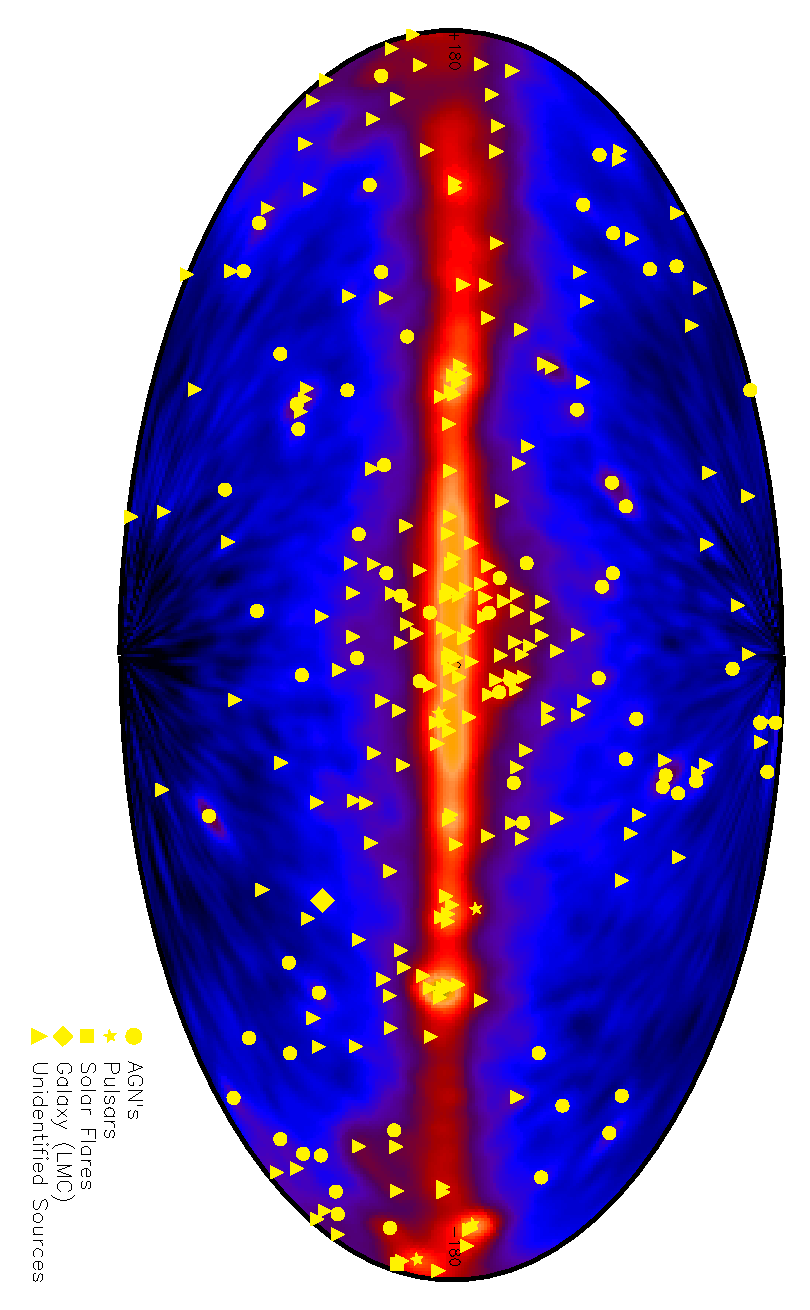
\includegraphics[width=0.8\columnwidth,angle=90]{Figures/3rd_egret_cat.eps} }
	\caption[Third EGRET catalog all-sky map.]{Third EGRET catalog all-sky map. Unidentified sources represented by triangles. Image courtesy of \url{https://heasarc.gsfc.nasa.gov/docs/cgro/images/epo/gallery/skymaps/}}
	\label{fig:3EGSky} 
\end{figure}

In spite of the difficulties in \egret{} source association, many studies have attempted correlating the unidentified \egret{} sources with various Galactic populations. In particular, several authors found strong evidence for statistical correlation between \glspl{snr} and some of the low-latitude unidentified sources \citep{Sturner95, Esposito96, Romero99}. In a review of the state of potential \snr{} /  \egret{} associations, \cite{Torres03} showed that there were 19 unidentified \egret{} sources that had an \snr~fall within its 95\% error box. Performing Monte Carlo simulations of the population of  \egret~sources, they determined that the chance probability for the 19 sources to be coincident with an \snr~was $1.05 \times 10^{-5}$, implying a probability of 0.99998 that at least one of the associations is real. Despite the statistical correlation of \egret~sources with \glspl{snr}, there were no definitive associations of an \snr~with any \egret~sources.

As the successor to \egret{}, the \lat{} was designed to improve upon its predecessor in a multitude of areas relevant to detecting \snrs{} \citep{atwood09,lat_perf}. The \lat{} has a much improved angular resolution (68\% single-photon containment radius $\sim 0.4^{\circ}$ at 1\gev{} for photons with the best quality direction reconstruction, PSF3 event type, compared to $\sim 1.7^{\circ}$ for \egret{} at the same energy), necessary to resolve \snrs{} as extended objects. The \lat{} also benefits from a superior sensitivity due to a combination of the improved \psf, larger peak effective area ($ {\rm > 9000~cm^2}$ vs. ${\rm \sim 1500~cm^2}$), wider \fov{} (2.4 sr, which is nearly 5 times that of \egret{}), and deeper, more-uniform sky exposure (afforded by the \lat's scanning observations as opposed to \egret's pointing operation). 

This bump in sensitivity results in the \lat{} detecting considerably more sources than \egret. Remarkably, within its first three months of commission, the \lat{} detected 205 sources above {\rm 10$\sigma$ significance \citep{lat_3m}, and by 11 months, 1451 sources above 4$\sigma$ \citep{1FGL}, compared to  the aforementioned 271 over the entire \egret{} mission. In fact, over its lifetime, \egret{} detected a total of about ${\rm 1.5~x~10^6}$ cosmic photons \citep{Thomson93}, while as of March 2016, the \lat{} has detected ${\rm \sim 863~x~10^6}$ \jamie{change this number in June} source class photons. The \lat's point-source sensitivity peaks between 1 and 10\gev{}, depending on location on the sky. With its increased sensitivity and higher energy range (up to $\sim$ 2\tev{} with the recent Pass 8 event reconstruction improvements, which is nearly an order of magnitude higher than \egret{}), the \lat{} is uniquely situated to study the \gam{} morphology and spectra of \snrs{}.
	
Both energetic lepton interactions (\ie \ic{} radiation of relativistic electrons interacting with ambient photon fields, and nonthermal \brems{}) and hadronic processes ($\pi_0$ decay \gam{}s from \cray{} protons encountering surrounding nuclei) produce spectra observable at \gam{} energies (see Chapter \ref{chap:gamAstr} for details). While the \ic{} generating electron population is also observable through emission of radio \sync{} photons, the proton-proton interaction solely emits \gam{}s. Despite being the prime energy range to observe the effects of cosmic particle acceleration, complexities at the lower \lat{} energy range stymie \snr{} morphology studies.
	
The \lat{} detects a strong, soft band of diffuse emission in the Galactic plane due to the interactions of  \crs{} with interstellar material. This bright diffuse radiation combined with the multiple potential emission scenarios, broadening \psf{} at decreasing energy, and a high source density in the plane can make it difficult to spatially disentangle sources observed by the \lat{}. To circumvent these 
difficulties, the majority of the analyses undertaken in this thesis are focused on the ${\rm E \geq 1\gev}$ energy range. This energy band is ideal for probing the properties of the accelerated particle populations present in the \snr{} environment. Studies of  \snrs{}  above 1\gev{} benefit from finer \lat{} \psf{}, striking a balance between minimizing the diffuse contribution, maximizing photon sensitivity, and retaining good photon statistics. Furthermore, evolved \snrs{}  exhibit a spectral break between 1-10\gev{} \citep{Hewitt15}. Explanations for the break range from Alfv\' en wave evanescence generated by collisions of partially ionized material in \mcs{} overtaken by \snr{}  shocks \citep{Malkov11}, reflected shocks in clouds \cite{Inoue10c}, and energy-dependent diffusion from shocks \cite{Ohira11}. Studying \snrs{} in this energy range hones our capability to tackle several goals set out by the \Fermi{} team when the mission was conceived.

\snr{I need to end with something about how/why awesome \Fermi{} has and will continue to be in searching for SNRs?mmaybe}
\section{Summary}\label{Rems:summ} In this section we summarized the end phase of stellar evolution (just enough to motivate SNRs) and descried the environs surrounding the supernova; development and phases of \glspl{snr} (and \glspl{pwn}?).  In particular we detailed the nonthermal emission mechanisms that produce \g-ray radiation, detection of young vs middle-aged( evolved, interacting with surroundings/dense medium),TeV detects younger typically, the troubles of detecting extension from them(?) something about different emission zones? Troubles disentangling hadronic from leptonic at \g-rays. \g-ray spectral and morphological features. Trends across the population wrt spectral shape/breaks, higher luminosity for interacting rems. Cosmic rays, using gamma-rays to probe CR population. So much of \g-ray astro is really about studying CRs, how much to say about them? 

\section{Scratch}
This chapter needs a different title. It's more focused on the specific sources being studied in this thesis. Galactic extended sources, SNRs, PWNe, but as in the SNRcat, not just extended SNRs, point-like SNRs as well.

Less focus on PWNe. Only give as much as I feel I need to support mentioning them a bit for 2FHL?

The focus of this section is supernova remnants in a gamma-ray context. Theory of evolution, what the gamma-ray emission is like, what we can learn from them individually.  This leads to the 1st SNR cat section for what we can do with them ensemble

NOt sure I really need any PWN stuff yet

in 2FHL we detect some pwn. If including above 10gev work, they'll be there too. Much of the thesis is really about extended gamma-ray sources, but not sure how that fits into the title and chapters yet

Do I need to get into composite SNRs (composite means SNR + PWN ) Maybe relevant for G150? Some things about interaction of reverse shock with PWN and crushing/reverberations of the PWN?

\cite{Montmerle79}